\documentclass[15pt]{article}

% Language setting
% Replace `english' with e.g. `spanish' to change the document language
\usepackage[english]{babel}
\usepackage{graphicx}
\graphicspath{ {./images/} }
% Set page size and margins
% Replace `letterpaper' with `a4paper' for UK/EU standard size

\usepackage[letterpaper,top=2cm,bottom=2cm,left=3cm,right=3cm,marginparwidth=1.75cm]{geometry}

% Useful packages
\usepackage{amsmath}
\usepackage{graphicx}
\usepackage[colorlinks=true, allcolors=blue]{hyperref}

\title{TP3 Automatique}

\begin{document}
\maketitle

\begin{abstract}
\end{abstract}

\section{Precision et performance des systemes asservis}

b) Il y'a un integrateur dans la fonction de transfert, on conjoncture que l'erreur statique est nulle. 

La marge de phase $\delta\phi$ vaut $31.8° $ 

La marge de gain $MG$ vaut $ 14.75dB$

c) On note $\omega_p \approx 3$ la pulsation de coupure a laquelle la phase $\phi$ vaut $-180°$.
$20log(\frac{K}{\omega_p\sqrt{1+\omega_p^2}\sqrt{10+\omega_p^2}}) < 0$


Methode 2 : 

$\delta G = 15dB$
$
$ \delta K = 10^{\frac{15}{20}} = 5.6$
$  Kmax = K * 5.6 = 20 * 5.6 = 112$



\title{Marge de gain et de phase de la fonction de transfert en boucle ouverte}


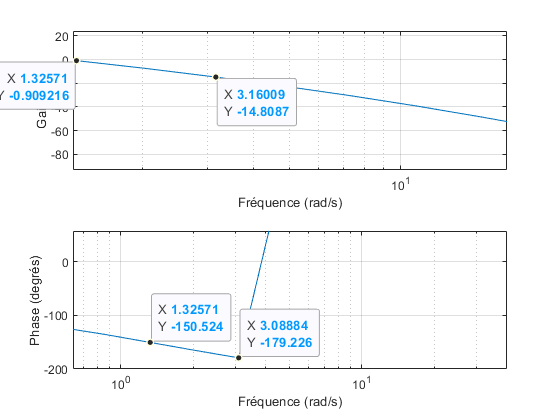
\includegraphics{marges_de_gain_phase.png}


\end{document}
	
